\documentclass{article}

\usepackage{amsmath,amssymb}
\usepackage{tikz}
\usepackage{pgfplots}
\usepackage{xcolor}
\usepackage[left=2.1cm,right=3.1cm,bottom=3cm,footskip=0.75cm,headsep=0.5cm]{geometry}
\usepackage{enumerate}
\usepackage{enumitem}
\usepackage{marvosym}
\usepackage{tabularx}
\usepackage[amsmath,thmmarks,standard]{ntheorem}
\usepackage{mathtools}

\usepackage[utf8]{inputenc}

\renewcommand*{\arraystretch}{1.4}
\newcommand{\E}{\mathbb{E}}

\newcolumntype{L}[1]{>{\raggedright\arraybackslash}p{#1}}
\newcolumntype{R}[1]{>{\raggedleft\arraybackslash}p{#1}}
\newcolumntype{C}[1]{>{\centering\let\newline\\\arraybackslash\hspace{0pt}}m{#1}}

\DeclareMathOperator{\tr}{tr}
\DeclareMathOperator{\Var}{Var}
\DeclareMathOperator{\Cov}{Cov}
\renewcommand{\E}{\mathbb{E}}

\newtheorem{thm}{Theorem}
\newtheorem{lem}{Lemma}

\title{\textbf{Einführung in die Produktion, Tutorium 8}}
\author{\textsc{Henry Haustein}}
\date{}

\begin{document}
	\maketitle
	
	\section*{Aufgabe 16}
	\begin{enumerate}[label=(\alph*)]
		\item kürzeste Gesamtbearbeitungszeit
		\begin{center}
			\begin{tabular}{c|c|c|c|c}
				\textbf{Reihenfolge} & \textbf{Bearbeitungszeit} & \textbf{Durchlaufzeit} & \textbf{Liefertermin} & \textbf{Verspätung} \\
				\hline
				C & 15 & 15 & 31 & 0 \\
				D & 19 & 34 & 25 & 9 \\
				B & 22 & 56 & 39 & 17 \\
				A & 25 & 81 & 42 & 39 \\
				\hline
				& 81 & & & 39
			\end{tabular}
		\end{center}
		\item Verfahren von Johnson
		\begin{center}
			\begin{tabular}{c|c|c|c||c|c||cccc}
				& \multicolumn{3}{c||}{\textbf{Bearbeitungsmatrix}} & \multicolumn{2}{c||}{\textbf{mod. Matrix}} & \multicolumn{4}{c}{\textbf{Reihenfolge}} \\
				\textbf{Auftrag} & $A_1$ & $A_2$ & $A_3$ & $A_1^\ast$ & $A_2^\ast$ & 1 & 2 & 3 & 4 \\
				\hline
				A & 14 & 5 & 6 & 19 & 11 & & & A$^3$ & \\
				B & 9 & 3 & 10 & 12 & 13 & & B$^4$ & & \\
				C & 8 & 1 & 6 & 9 & 7 & & & & C$^1$ \\
				D & 3 & 5 & 11 & 8 & 16 & D$^2$ & & &
			\end{tabular}
		\end{center}
		\item Eine der folgenden beiden Bedingungen muss erfüllt sein, dann ist das 3-Maschinen-Problem auf ein 2-Maschinen-Problem reduzierbar und das Verfahren von Johnson liefert eine optimale Lösung:
		\begin{itemize}
			\item $t_{p_{2,max}} \le t_{p_{1,min}}$: $5\not\le 3$
			\item $t_{p_{2,max}} \le t_{p_{3,min}}$: $5\le 6$
		\end{itemize}
		Das Verfahren von Johnson liefert eine optimale Lösung.
		\item Gantt-Diagramm
		\begin{center}
			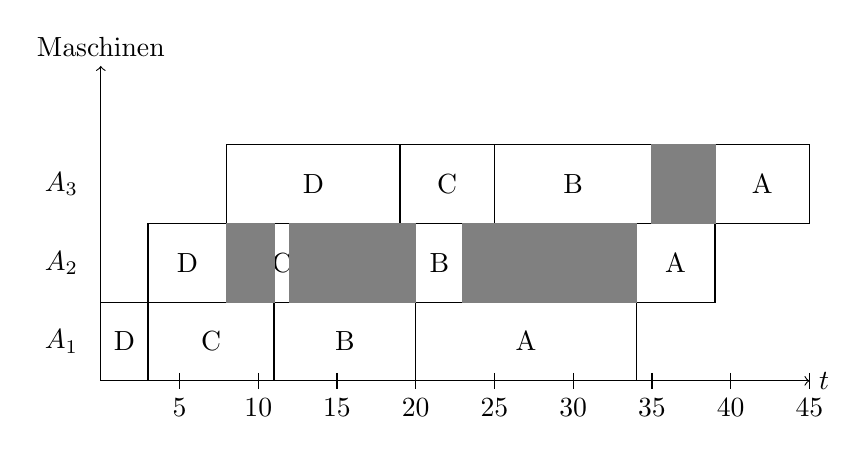
\begin{tikzpicture}
				\draw[->] (0,0) to (45/5,0) node[right] {$t$};
				\draw[->] (0,0) to (0,4) node[above] {Maschinen};
				
				\foreach \x in {5,10,15,20,25,30,35,40,45} {
					\draw (\x/5,0.1) to (\x/5,-0.1) node[below] {\x};
				}
				
				\node at (-0.5,0.5) {$A_1$};
				\node at (-0.5,1.5) {$A_2$};
				\node at (-0.5,2.5) {$A_3$};
				
				\draw (0,0) rectangle (3/5,1) node[pos=0.5] {D};
				\draw (3/5,0) rectangle (11/5,1) node[pos=0.5] {C};
				\draw (11/5,0) rectangle (20/5,1) node[pos=0.5] {B};
				\draw (20/5,0) rectangle (34/5,1) node[pos=0.5] {A};
				
				\draw (3/5,1) rectangle (8/5,2) node[pos=0.5] {D};
				\draw (11/5,1) rectangle (12/5,2) node[pos=0.5] {C};
				\draw (20/5,1) rectangle (23/5,2) node[pos=0.5] {B};
				\draw (34/5,1) rectangle (39/5,2) node[pos=0.5] {A};
				
				\draw (8/5,2) rectangle (19/5,3) node[pos=0.5] {D};
				\draw (19/5,2) rectangle (25/5,3) node[pos=0.5] {C};
				\draw (25/5,2) rectangle (35/5,3) node[pos=0.5] {B};
				\draw (39/5,2) rectangle (45/5,3) node[pos=0.5] {A};
				
				\draw[gray,fill=gray] (8/5,1) rectangle (11/5,2);
				\draw[gray,fill=gray] (12/5,1) rectangle (20/5,2);
				\draw[gray,fill=gray] (23/5,1) rectangle (34/5,2);
				
				\draw[gray,fill=gray] (35/5,2) rectangle (39/5,3);
			\end{tikzpicture}
		\end{center}
		Die Zykluszeit ist 45 und die Summe der Leerzeiten ist 3 + 8 + 11 + 4 = 26.
	\end{enumerate}
	
\end{document}